% Document/LinearAlgebra/VectorSpaces/QuotientSpaces/Construction.tex
% Phase 11: Quotient Space Construction and Universal Property

\newpage
\section{Quotient Space Construction}

\begin{intuition}[Chapter Overview]
    Subspaces are the substructures of a vector space; quotient spaces are the
    \textbf{factor structures}. Given a subspace $W \Subspace[K] V$, the quotient
    $\QuotientSpace{V}{W}$ is the vector space obtained by ``collapsing $W$ to zero'' ---
    declaring two vectors equivalent if they differ by an element of $W$. The resulting
    equivalence classes (cosets $v + W$) inherit well-defined vector space operations, and the
    canonical projection $\pi: V \to \QuotientSpace{V}{W}$ is a surjective linear map whose
    kernel is exactly $W$.

    Quotient spaces serve two fundamental roles:
    \begin{itemize}
        \item \textbf{Factoring linear maps.} Every linear map $T: V \to X$ with
              $W \subseteq \Ker{T}$ factors uniquely through $\QuotientSpace{V}{W}$. This
              universal property makes quotients the natural tool for analyzing maps by
              ``dividing out'' their kernel.
        \item \textbf{Structural theorems.} The four isomorphism theorems --- direct analogues
              of the classical theorems for groups and rings --- describe how subspaces, sums,
              intersections, and nested quotients interact. These theorems reduce complex
              structural questions to manageable calculations.
    \end{itemize}

    Geometrically, if $V = \bb{R}^3$ and $W$ is a plane through the origin, the quotient
    $\QuotientSpace{V}{W}$ is a one-dimensional space whose ``points'' are the planes parallel
    to $W$. Each coset $v + W$ is a translate of $W$, and the quotient records only how far a
    vector is displaced from $W$ in the transverse direction.
\end{intuition}

\begin{remark}[Intuition]
    Given a subspace $W \Subspace[K] V$, we want to build a new vector space in which
    every vector in $W$ becomes zero --- we ``collapse'' $W$ to a single point. The price
    is that we can no longer distinguish vectors that differ only by an element of $W$: if
    $u - v \in W$, then $u$ and $v$ become the same object in the quotient. The equivalence
    classes $v + W = \{v + w \mid w \in W\}$ are the \textbf{cosets} of $W$, and they are
    the ``points'' of the quotient space $\QuotientSpace{V}{W}$.

    Geometrically, each coset is a translate of $W$ --- a parallel copy of the subspace
    $W$ displaced by the vector $v$. The quotient space is the set of all such parallel
    copies, equipped with natural addition and scalar multiplication defined through
    representatives. For instance:
    \begin{itemize}
        \item If $V = \bb{R}^2$ and $W$ is a line through the origin, the cosets are lines
              parallel to $W$. The quotient $\QuotientSpace{\bb{R}^2}{W}$ is one-dimensional:
              it parameterizes how far a point is from $W$ in the transverse direction.
        \item If $V = \bb{R}^3$ and $W$ is a plane through the origin, the cosets are planes
              parallel to $W$, and $\QuotientSpace{\bb{R}^3}{W} \cong \bb{R}$.
        \item If $V = K[X]$ and $W = \Span[K]{\{X^n \mid n \geq 2\}}$, the quotient
              identifies two polynomials that agree up to degree $1$ --- it retains only the
              constant and linear terms.
    \end{itemize}
    The key technical point is \textbf{well-definedness}: the operations on cosets must not
    depend on which representative we choose. This is exactly where the hypothesis that $W$
    is a subspace (not just a subset) is used.
\end{remark}

\begin{definition}[Quotient Equivalence Relation]\label{def:quotient-equiv}
    Let $W \Subspace[K] V$. Define an equivalence relation on $V$ by:
    \[
        u \sim_W v \quad \Leftrightarrow \quad u - v \in W
    \]
    The equivalence class of $v$ is the \textbf{coset} $\Coset{v}{W} = \Set{v + w \mid w \in W}$.
\end{definition}

\begin{proposition}[Equivalence Relation and Cosets]\label{prop:quotient-equiv}
    The relation $\sim_W$ is an equivalence relation on $V$, and the equivalence class of $v$
    is the coset $v + W = \Set{v + w \mid w \in W}$ for any $v \in V$.
\end{proposition}

\begin{proof}
    We verify the three properties:
    \begin{itemize}
        \item \textbf{Reflexivity}: $v - v = 0 \in W$, so $v \sim_W v$.
        \item \textbf{Symmetry}: If $u - v \in W$, then $v - u = -(u - v) \in W$ since $W$ is a subspace.
        \item \textbf{Transitivity}: If $u - v \in W$ and $v - w \in W$, then 
              $u - w = (u - v) + (v - w) \in W$ since $W$ is closed under addition.
    \end{itemize}
    
    \textbf{Equivalence class equals coset:}
    Let $\EquivClass{v}$ denote the equivalence class of $v$ and $v + W = \Set{v + w \mid w \in W}$.
    \begin{align*}
        u \in \EquivClass{v} &\Leftrightarrow u \sim_W v \\
                              &\Leftrightarrow u - v \in W \\
                              &\Leftrightarrow \Exists :{w \in W}{u - v = w} \\
                              &\Leftrightarrow \Exists :{w \in W}{u = v + w} \\
                              &\Leftrightarrow u \in v + W
    \end{align*}
    Thus $\EquivClass{v} = v + W$.
\end{proof}

\begin{definition}[Quotient Space]\label{def:quotient-space}
    Let $W \Subspace[K] V$. The \textbf{quotient space} $\QuotientSpace{V}{W}$ is the set of
    all cosets of $W$ in $V$:
    \[
        \QuotientSpace{V}{W} = \Set{\Coset{v}{W} \mid v \in V}
        = \Set{\EquivClass{v} \mid v \in V}
    \]
    We write $\Coset{v}{W}$ (coset notation) and $\EquivClass{v}$ (equivalence class notation)
    interchangeably for the same element of $\QuotientSpace{V}{W}$.

    The vector space operations are defined through representatives:
    \begin{align*}
        \Coset{u}{W} + \Coset{v}{W} &= \Coset{(u + v)}{W}
        &\quad\text{i.e.,}\quad
        \EquivClass{u} + \EquivClass{v} &= \EquivClass{u + v} \\
        a \cdot \Coset{v}{W} &= \Coset{(av)}{W}
        &\quad\text{i.e.,}\quad
        a \cdot \EquivClass{v} &= \EquivClass{av}
    \end{align*}
    for all $u, v \in V$ and $a \in K$.
    More generally, $a\EquivClass{u} + b\EquivClass{v} = \EquivClass{au + bv}$.
\end{definition}

\begin{theorem}[Vector Space Structure]\label{thm:quotient-vs}
    The operations on $\QuotientSpace{V}{W}$ are well-defined, and $\QuotientSpace{V}{W}$
    is a $K$-vector space.
\end{theorem}

\begin{proof}
    \textbf{Well-definedness of addition:}
    Suppose $\Coset{u_1}{W} = \Coset{u_2}{W}$ and $\Coset{v_1}{W} = \Coset{v_2}{W}$,
    i.e., $u_1 - u_2 \in W$ and $v_1 - v_2 \in W$.
    Then $(u_1 + v_1) - (u_2 + v_2) = (u_1 - u_2) + (v_1 - v_2) \in W$,
    so $\Coset{(u_1 + v_1)}{W} = \Coset{(u_2 + v_2)}{W}$.
    
    \textbf{Well-definedness of scalar multiplication:}
    Suppose $\Coset{v_1}{W} = \Coset{v_2}{W}$, i.e., $v_1 - v_2 \in W$.
    Then $av_1 - av_2 = a(v_1 - v_2) \in W$ since $W$ is a subspace.
    Thus $\Coset{(av_1)}{W} = \Coset{(av_2)}{W}$.
    
    \textbf{Vector space axioms:}
    The axioms follow from those of $V$ via representatives. For example:
    \begin{itemize}
        \item Zero element: $\EquivClass{0} = \Coset{0}{W} = W$ satisfies
              $\EquivClass{v} + \EquivClass{0} = \EquivClass{v+0} = \EquivClass{v}$.
        \item Additive inverse: $-\EquivClass{v} = \EquivClass{-v}$ since
              $\EquivClass{v} + \EquivClass{-v} = \EquivClass{0}$.
        \item Associativity, commutativity, distributivity all follow by computing with representatives
              and using well-definedness.
    \end{itemize}
\end{proof}

\begin{definition}[Canonical Projection]\label{def:canonical-proj}
    The \textbf{canonical projection} (or \textbf{quotient map}) is the linear map:
    \[
        \pi: V \to \QuotientSpace{V}{W}, \quad \pi(v) = \Coset{v}{W} = \EquivClass{v}
    \]
\end{definition}

\begin{proposition}[Properties of Canonical Projection]\label{prop:canonical-proj}
    The canonical projection $\pi: V \to \QuotientSpace{V}{W}$ satisfies:
    \begin{enumerate}
        \item $\pi$ is linear
        \item $\pi$ is surjective
        \item $\Ker{\pi} = W$
    \end{enumerate}
\end{proposition}

\begin{proof}
    \textbf{(1) Linearity:}
    For $u, v \in V$ and $a, b \in K$:
    \[
        \pi(au + bv) = \EquivClass{au + bv} = a\EquivClass{u} + b\EquivClass{v} = a\pi(u) + b\pi(v)
    \]

    \textbf{(2) Surjectivity:}
    Every element of $\QuotientSpace{V}{W}$ has the form $\EquivClass{v} = \pi(v)$ for some $v \in V$.

    \textbf{(3) Kernel:}
    \begin{align*}
        v \in \Ker{\pi} &\Leftrightarrow \pi(v) = \EquivClass{0} \\
                        &\Leftrightarrow \EquivClass{v} = \EquivClass{0} \\
                        &\Leftrightarrow v - 0 \in W \\
                        &\Leftrightarrow v \in W
    \end{align*}
\end{proof}

\newpage
\section{Examples of Quotient Spaces}

\begin{example}[$\bb{R}^2$ Quotient by a Line]\label{ex:quotient-r2-line}
    Let $V = \bb{R}^2$ and $L = \Span[\bb{R}]{\Set{(1, 1)}}$ be the line $y = x$ through the origin.
    
    The cosets are parallel lines: for any $(a, b) \in \bb{R}^2$,
    \[
        \Coset{(a, b)}{L} = \Set{(a + t, b + t) \mid t \in \bb{R}}
    \]
    This is the line $y = x + (b - a)$.
    
    Two points $(a_1, b_1)$ and $(a_2, b_2)$ are in the same coset iff $b_1 - a_1 = b_2 - a_2$,
    i.e., iff they have the same ``signed distance'' from the line $L$.
    
    The quotient $\QuotientSpace{\bb{R}^2}{L}$ is 1-dimensional, isomorphic to $\bb{R}$
    via the map $\Coset{(a, b)}{L} \mapsto b - a$.
    
    \begin{center}
    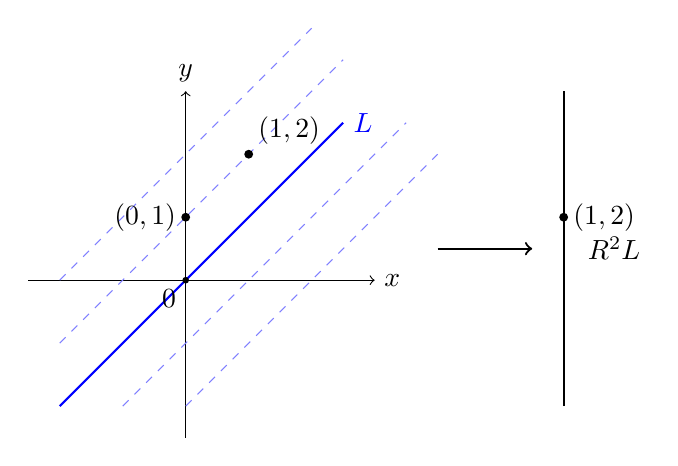
\begin{tikzpicture}[scale=0.8]
        % Coordinate axes
        \draw[->] (-2.5,0) -- (3,0) node[right] {$x$};
        \draw[->] (0,-2.5) -- (0,3) node[above] {$y$};
        
        % Line L (y = x)
        \draw[blue, thick] (-2,-2) -- (2.5,2.5) node[right] {$L$};
        
        % Parallel cosets
        \draw[blue!50, dashed] (-2,-1) -- (2.5,3.5);
        \draw[blue!50, dashed] (-2,0) -- (2,4);
        \draw[blue!50, dashed] (-1,-2) -- (3.5,2.5);
        \draw[blue!50, dashed] (0,-2) -- (4,2);
        
        % Points and labels
        \fill (1,2) circle (2pt) node[above right] {$(1,2)$};
        \fill (0,1) circle (2pt) node[left] {$(0,1)$};
        
        % Origin
        \fill (0,0) circle (1.5pt) node[below left] {$0$};
        
        % Arrow to quotient
        \draw[->, thick] (4,0.5) -- (5.5,0.5);
        
        % 1D quotient space
        \draw[thick] (6,-2) -- (6,3);
        \node at (6.8,0.5) {$\QuotientSpace{\bb{R}^2}{L}$};
        \fill (6,1) circle (2pt) node[right] {$\EquivClass{(1,2)}$};
    \end{tikzpicture}
    \end{center}
\end{example}

\begin{example}[$\bb{R}^3$ Quotient by a Plane]\label{ex:quotient-r3-plane}
    Let $V = \bb{R}^3$ and $P = \Set{(x, y, 0) \mid x, y \in \bb{R}}$ be the $xy$-plane.
    
    The cosets are planes parallel to $P$: for any $(a, b, c) \in \bb{R}^3$,
    \[
        \Coset{(a, b, c)}{P} = \Set{(a + s, b + t, c) \mid s, t \in \bb{R}}
    \]
    This is the plane at height $z = c$.
    
    Two points are in the same coset iff they have the same $z$-coordinate.
    The quotient $\QuotientSpace{\bb{R}^3}{P}$ is 1-dimensional, isomorphic to $\bb{R}$ 
    (the $z$-axis) via $\Coset{(a,b,c)}{P} \mapsto c$.
    
    \begin{center}
    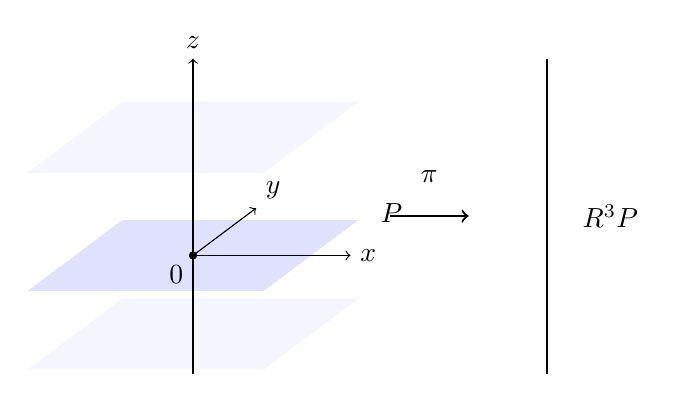
\begin{tikzpicture}[scale=1.0,
        x={(1cm,0cm)},
        y={(0.4cm,0.3cm)},
        z={(0cm,1cm)}]
        
        % xy-plane (P)
        \fill[blue!20, opacity=0.6] (-1.5,-1.5,0) -- (1.5,-1.5,0) -- (1.5,1.5,0) -- (-1.5,1.5,0) -- cycle;
        \node at (1.8,1.8,0) {$P$};
        
        % Parallel planes (cosets)
        \fill[blue!10, opacity=0.4] (-1.5,-1.5,1.5) -- (1.5,-1.5,1.5) -- (1.5,1.5,1.5) -- (-1.5,1.5,1.5) -- cycle;
        \fill[blue!10, opacity=0.4] (-1.5,-1.5,-1) -- (1.5,-1.5,-1) -- (1.5,1.5,-1) -- (-1.5,1.5,-1) -- cycle;
        
        % Coordinate axes
        \draw[->] (0,0,0) -- (2,0,0) node[right] {$x$};
        \draw[->] (0,0,0) -- (0,2,0) node[above right] {$y$};
        \draw[->] (0,0,-1.5) -- (0,0,2.5) node[above] {$z$};
        
        % Origin
        \fill (0,0,0) circle (1.5pt) node[below left] {$0$};
        
        % Arrow to quotient
        \draw[->, thick] (2.5,0,0.5) -- (3.5,0,0.5);
        \node at (3,0,1) {$\pi$};
        
        % 1D quotient (z-axis representation)
        \draw[thick] (4.5,0,-1.5) -- (4.5,0,2.5);
        \node at (5.3,0,0.5) {$\QuotientSpace{\bb{R}^3}{P}$};
    \end{tikzpicture}
    \end{center}
\end{example}

\begin{example}[Polynomials mod $X^2$]\label{ex:quotient-poly}
    Let $V = K[X]$ and $W = \Span[K]{\Set{X^n \mid n \geq 2}}$ be the subspace of 
    polynomials with zero constant and linear terms.
    
    Two polynomials $p, q \in K[X]$ satisfy $p \sim_W q$ iff $p - q \in W$,
    i.e., iff $p$ and $q$ have the same constant and linear coefficients.
    
    Each coset is determined by its ``remainder modulo $X^2$'':
    \[
        \Coset{(a_0 + a_1 X + a_2 X^2 + \cdots)}{W} = \Coset{(a_0 + a_1 X)}{W}
    \]
    
    The quotient space has basis $\Set{\EquivClass{1}, \EquivClass{X}}$, so $\Dim[K]{\QuotientSpace{K[X]}{W}} = 2$.
\end{example}

\newpage
\section{Dimension of Quotient Spaces}

\begin{remark}[Motivation]
    Since $\QuotientSpace{V}{W}$ is obtained by collapsing a $\Dim{W}$-dimensional piece
    of $V$ to zero, we expect the quotient to have dimension $\Dim{V} - \Dim{W}$. The
    quotient dimension formula makes this precise: $\Dim{W} + \Dim{\QuotientSpace{V}{W}} = \Dim{V}$.
    This is stated in additive form so that it is valid even when the dimensions are infinite
    cardinals, where subtraction may not be meaningful.

    The proof is constructive: start with a basis for $W$, extend it to a basis for $V$,
    and show that the cosets of the extension vectors form a basis for the quotient. This
    is the same ``extend and project'' strategy used in the direct proof of rank-nullity
    (Theorem~\ref{thm:rank-nullity}), and the resemblance is not coincidental --- the
    first isomorphism theorem will show that rank-nullity is a corollary of the quotient
    dimension formula.
\end{remark}

\begin{theorem}[Quotient Dimension Formula]\label{thm:quotient-dim}
    Let $W \Subspace[K] V$. Then:
    \[
        \Dim[K]{W} + \Dim[K]{\QuotientSpace{V}{W}} = \Dim[K]{V}
    \]
    In particular, for finite-dimensional $V$:
    \[
        \Dim[K]{\QuotientSpace{V}{W}} = \Dim[K]{V} - \Dim[K]{W}
    \]
\end{theorem}

\begin{proof}
    Let $B_W = \Set{w_i}_{i \in I}$ be a basis for $W$.
    By the Basis Extension Theorem (Theorem~\ref{thm:basis-extension}), extend $B_W$ to a 
    basis $B = B_W \Union \Set{v_j}_{j \in J}$ for $V$, where $B_W \Intersect \Set{v_j}_{j \in J} = \emptyset$.
    
    We claim that $\Set{\EquivClass{v_j}}_{j \in J}$ is a basis for $\QuotientSpace{V}{W}$.
    
    \textbf{Generating:}
    Let $\EquivClass{v} \in \QuotientSpace{V}{W}$ with $v = \sum_{i \in F_1} a_i w_i + \sum_{j \in F_2} b_j v_j$
    for finite $F_1 \subseteq I$, $F_2 \subseteq J$.
    Then:
    \[
        \EquivClass{v} = \EquivClass{\sum_{i \in F_1} a_i w_i + \sum_{j \in F_2} b_j v_j} 
                       = \sum_{i \in F_1} a_i \EquivClass{w_i} + \sum_{j \in F_2} b_j \EquivClass{v_j}
                       = \sum_{j \in F_2} b_j \EquivClass{v_j}
    \]
    since $\EquivClass{w_i} = \EquivClass{0}$ for all $w_i \in W$.
    
    \textbf{Linear independence:}
    Suppose $\sum_{j \in F} b_j \EquivClass{v_j} = \EquivClass{0}$ for some finite $F \subseteq J$.
    Then $\EquivClass{\sum_{j \in F} b_j v_j} = \EquivClass{0}$, which means $\sum_{j \in F} b_j v_j \in W$.
    
    Write $\sum_{j \in F} b_j v_j = \sum_{i \in G} a_i w_i$ for some finite $G \subseteq I$.
    Rearranging: $\sum_{j \in F} b_j v_j - \sum_{i \in G} a_i w_i = 0$.
    
    Since $B$ is linearly independent and $\Set{w_i}_{i \in G} \Union \Set{v_j}_{j \in F} \subseteq B$,
    all coefficients must be zero. In particular, all $b_j = 0$.
    
    Thus $\Set{\EquivClass{v_j}}_{j \in J}$ is a basis for $\QuotientSpace{V}{W}$, hence:
    \[
        \Card{B_W} + \Dim[K]{\QuotientSpace{V}{W}} = \Card{B_W} + \Card{J} = \Card{B}
    \]
    That is, $\Dim[K]{W} + \Dim[K]{\QuotientSpace{V}{W}} = \Dim[K]{V}$.
    
    In finite dimensions, we can subtract to obtain $\Dim[K]{\QuotientSpace{V}{W}} = \Dim[K]{V} - \Dim[K]{W}$.
\end{proof}

\newpage
\section{Universal Property of Quotient Spaces}

\begin{remark}[Motivation]
    The universal property of quotient spaces is the dual of the universal property of free
    vector spaces (Theorem~\ref{thm:vector-space-universal}). Where the free property says
    ``maps \emph{out of} $V$ are determined by values on a basis,'' the quotient property
    says ``maps \emph{out of} $\QuotientSpace{V}{W}$ correspond exactly to maps out of $V$
    that kill $W$.''

    In categorical language, the canonical projection $\pi: V \to \QuotientSpace{V}{W}$ is
    the \textbf{cokernel} of the inclusion $W \hookrightarrow V$: it is the universal map
    that makes the inclusion zero. This universal characterization means that $\QuotientSpace{V}{W}$
    is determined up to unique isomorphism by the pair $(V, W)$ --- any other space with the
    same factoring property is canonically isomorphic to $\QuotientSpace{V}{W}$.

    In practice, the universal property is the main tool for constructing maps out of
    quotient spaces: rather than working with cosets directly, define a map on $V$, verify
    that it kills $W$, and invoke the theorem.
\end{remark}

The universal property characterizes the quotient space by its relationship to linear maps
whose kernel contains the subspace $W$.

\begin{center}
\begin{tikzcd}
V \arrow[r, "\pi"] \arrow[dr, "T"'] & \QuotientSpace{V}{W} \arrow[d, dashed, "\exists! \tilde{T}"] \\
 & X
\end{tikzcd}
\end{center}

\begin{theorem}[Universal Property of Quotient Spaces]\label{thm:quotient-universal}
    Let $W \Subspace[K] V$ and $T: V \to X$ be a linear map. Then:
    \begin{enumerate}
        \item There exists a linear map $\tilde{T}: \QuotientSpace{V}{W} \to X$ with 
              $T = \Composition{\tilde{T}}{\pi}$ if and only if $W \subseteq \Ker{T}$.
        \item If such $\tilde{T}$ exists, it is unique.
        \item $\tilde{T}$ is surjective if and only if $T$ is surjective.
        \item $\tilde{T}$ is injective if and only if $\Ker{T} = W$.
        \item $\tilde{T}$ is an isomorphism if and only if $T$ is surjective and $\Ker{T} = W$.
    \end{enumerate}
\end{theorem}

\begin{proof}
    \textbf{(1) Existence:}
    
    ($\Rightarrow$)
    Suppose $\tilde{T}$ exists with $T = \Composition{\tilde{T}}{\pi}$.
    Then:
    \[
        \Ker{T} = \Ker{\Composition{\tilde{T}}{\pi}} \supseteq \Ker{\pi} = W
    \]
    Thus $W \subseteq \Ker{T}$.
    
    ($\Leftarrow$)
    Suppose $W \subseteq \Ker{T}$. Define $\tilde{T}: \QuotientSpace{V}{W} \to X$ by:
    \[
        \tilde{T}(\Coset{v}{W}) = T(v)
    \]
    
    \textit{Well-defined:} If $\Coset{v_1}{W} = \Coset{v_2}{W}$, then $v_1 - v_2 \in W \subseteq \Ker{T}$.
    Thus $T(v_1) - T(v_2) = T(v_1 - v_2) = 0$, so $T(v_1) = T(v_2)$.
    
    \textit{Linear:} For $\Coset{u}{W}, \Coset{v}{W} \in \QuotientSpace{V}{W}$ and $a, b \in K$:
    \begin{align*}
        \tilde{T}(a\Coset{u}{W} + b\Coset{v}{W}) &= \tilde{T}(\Coset{au + bv}{W}) \\
                                                  &= T(au + bv) \\
                                                  &= aT(u) + bT(v) \\
                                                  &= a\tilde{T}(\Coset{u}{W}) + b\tilde{T}(\Coset{v}{W})
    \end{align*}
    
    \textit{Factorization:} For any $v \in V$: $\tilde{T}(\pi(v)) = \tilde{T}(\Coset{v}{W}) = T(v)$.
    Thus $\Composition{\tilde{T}}{\pi} = T$.
    
    \textbf{(2) Uniqueness:}
    Suppose $\tilde{T}_1$ and $\tilde{T}_2$ both satisfy $\Composition{\tilde{T}_1}{\pi} = T = \Composition{\tilde{T}_2}{\pi}$.
    
    Since $\pi$ is surjective (an epimorphism), and $\Composition{\tilde{T}_1}{\pi} = \Composition{\tilde{T}_2}{\pi}$,
    it follows that $\tilde{T}_1 = \tilde{T}_2$ by the cancellation property of epimorphisms.
    
    \textbf{(3) Surjectivity:}
    Since $T = \Composition{\tilde{T}}{\pi}$ and $\pi$ is surjective:
    \[
        \Rng{T} = \Rng{\Composition{\tilde{T}}{\pi}} = \DirectImage{\tilde{T}}{\Rng{\pi}} = \DirectImage{\tilde{T}}{\QuotientSpace{V}{W}} = \Rng{\tilde{T}}
    \]
    Thus $T$ is surjective if and only if $\tilde{T}$ is surjective.
    
    \textbf{(4) Injectivity:}
    
    ($\Rightarrow$)
    Suppose $\tilde{T}$ is injective (a monomorphism).
    We have $W \subseteq \Ker{T}$ by (1).
    Conversely, let $v \in \Ker{T}$. Then $\tilde{T}(\pi(v)) = T(v) = 0 = \tilde{T}(0)$.
    Since $\tilde{T}$ is a monomorphism, $\pi(v) = 0$, i.e., $v \in \Ker{\pi} = W$.
    Thus $\Ker{T} \subseteq W$, so $\Ker{T} = W$.
    
    ($\Leftarrow$)
    Suppose $\Ker{T} = W$. Let $\tilde{T}(\Coset{v_1}{W}) = \tilde{T}(\Coset{v_2}{W})$.
    Then $T(v_1) = T(v_2)$, so $v_1 - v_2 \in \Ker{T} = W$.
    Thus $\Coset{v_1}{W} = \Coset{v_2}{W}$, so $\tilde{T}$ is injective.
    
    \textbf{(5) Isomorphism:}
    Combine (3) and (4): $\tilde{T}$ is bijective (hence an isomorphism, by Theorem~\ref{thm:bijectivity})
    if and only if $T$ is surjective and $\Ker{T} = W$.
\end{proof}

\begin{remark}[Application of Universal Property]
    The universal property provides a systematic way to:
    \begin{enumerate}
        \item \textbf{Factor maps}: Given $T: V \to X$ with $W \subseteq \Ker{T}$,
              we can factor $T = \Composition{\tilde{T}}{\pi}$ through the quotient.
        \item \textbf{Construct maps out of quotients}: To define a linear map from $\QuotientSpace{V}{W}$,
              it suffices to define a map on $V$ that vanishes on $W$.
        \item \textbf{Identify when quotients are isomorphic}: $\QuotientSpace{V}{W} \cong X$ 
              iff there exists surjective $T: V \to X$ with $\Ker{T} = W$.
    \end{enumerate}
\end{remark}
